%!TeX root = KraetkeZiegenhagen_CI.tex
\section{Jenkins -- Installation und Nutzung}

In diesem Abschnitt möchte ich kurz zeigen, wie man Jenkins installieren und konfigurieren muss, um eigene \LaTeX-Dokumente damit zu übersetzen.

Jenkins bildet die Softwarebasis, die wir zur Steuerung des Build-Prozesses nutzen werden und wurde ursprünglich unter dem Namen \enquote{Hudson} bei Sun Microsystems entwickelt. Jenkins benötigt Java -- es basiert auf den sogenannten \enquote{Enterprise Java Beans} und wird über den Webbrowser bedient. 

Im folgenden beschreibe ich das Setup unter Ubuntu, es sind aber auch Installationspakete für Windows, Mac OS X und diverse Linux-Varianten verfügbar.

Die eigentliche Installation verläuft unspektakulär, siehe das folgende Listing. Bei den meisten Debian-basierten Linuxen dürfte ein \lstinline{apt-get update} mit anschließendem \lstinline{apt-get install jenkins} ausreichen, für meine Linux-Version Xubuntu \enquote{Yakkety Yak} gab es jedoch noch kein Paket, sodass ich das Debian Repository einbinden musste, siehe \url{https://pkg.jenkins.io/debian/}

\begin{lstlisting}{caption={jenkins Installation},label={lis:install}}
wget -q -O - https://pkg.jenkins.io/debian/jenkins.io.key | sudo apt-key add -
# deb https://pkg.jenkins.io/debian binary/ in 
# die Datei /etc/apt/sources.list mit aufnehmen
sudo apt-get update
sudo apt-get install jenkins
\end{lstlisting}

Nach der Installation -- ein Neustart ist nicht notwendig -- kann dann über Port 8080 des Installationsrechners auf die jenkins-Oberfläche zugegriffen werden. Im ersten Schritt müssen wir das Initial-Passwort aus einer Datei der jenkins-Installation kopieren, siehe Abbildung \ref{fig:initial}.

\begin{figure}
\fbox{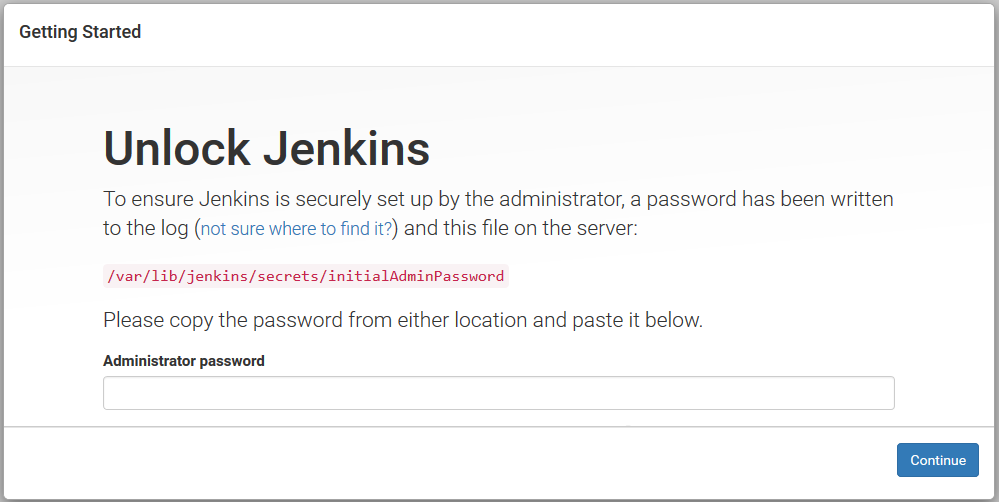
\includegraphics[width=\textwidth]{Images/Password}}
\caption{Festlegung des Initial-Passworts}\label{fig:initial}
\end{figure}

Im nächsten Schritt (siehe Abbildung \ref{fig:Plugins}) werden die Plugins ausgewählt, die wir benutzen möchten. Hier belasse ich es bei den Standard-Plugins, weitere lassen sich später nachinstallieren.

\begin{figure}
\fbox{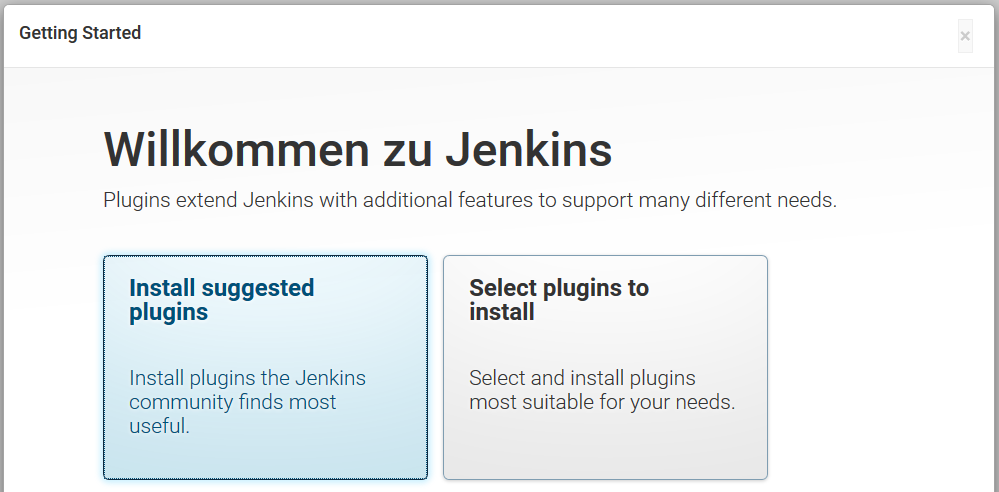
\includegraphics[width=\textwidth]{Images/Plugins}}
\caption{Auswahl der Plugins}\label{fig:Plugins}
\end{figure}


\begin{figure}
\fbox{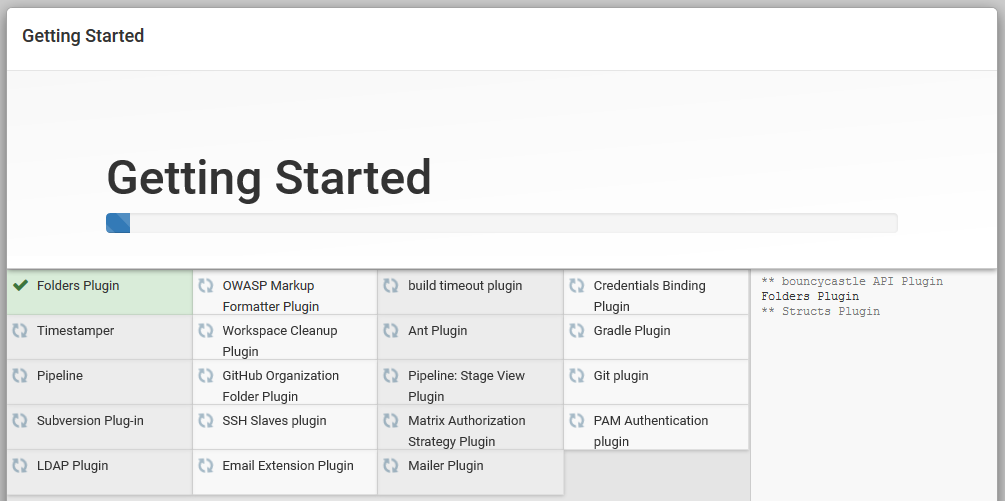
\includegraphics[width=\textwidth]{Images/Plugins2}}
\caption{Auswahl der Plugins}\label{fig:Plugins2}
\end{figure}

Nach der Erstellung eines Administratorkontos, siehe Abbildung \ref{fig:Admin}, können wir auf die Oberfläche zugreifen und neue Aufträge erstellen (siehe Abbildung \ref{fig:NewJob}).

\begin{figure}
\fbox{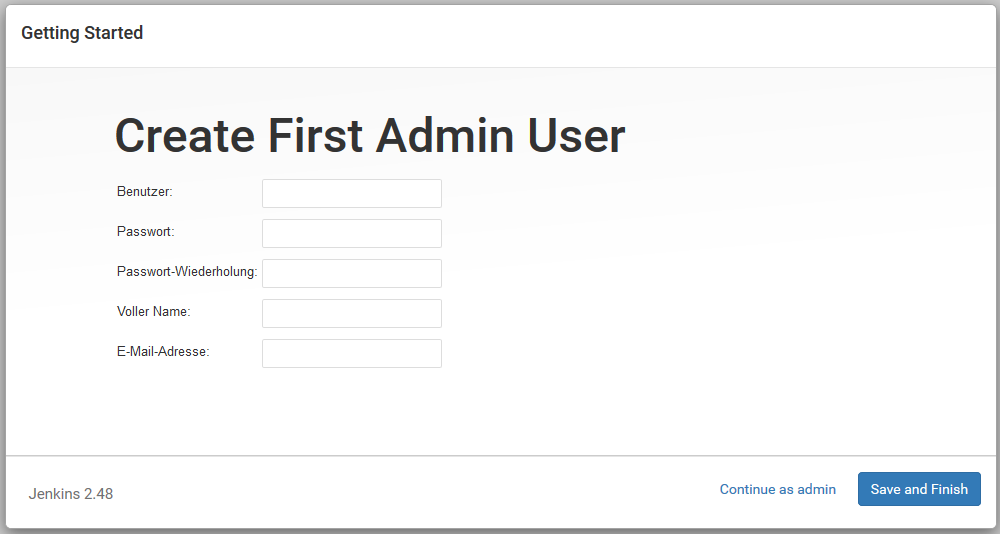
\includegraphics[width=\textwidth]{Images/Admin}}
\caption{Erstellung des Administrator-Kontos}\label{fig:Admin}
\end{figure}


\begin{figure}
\fbox{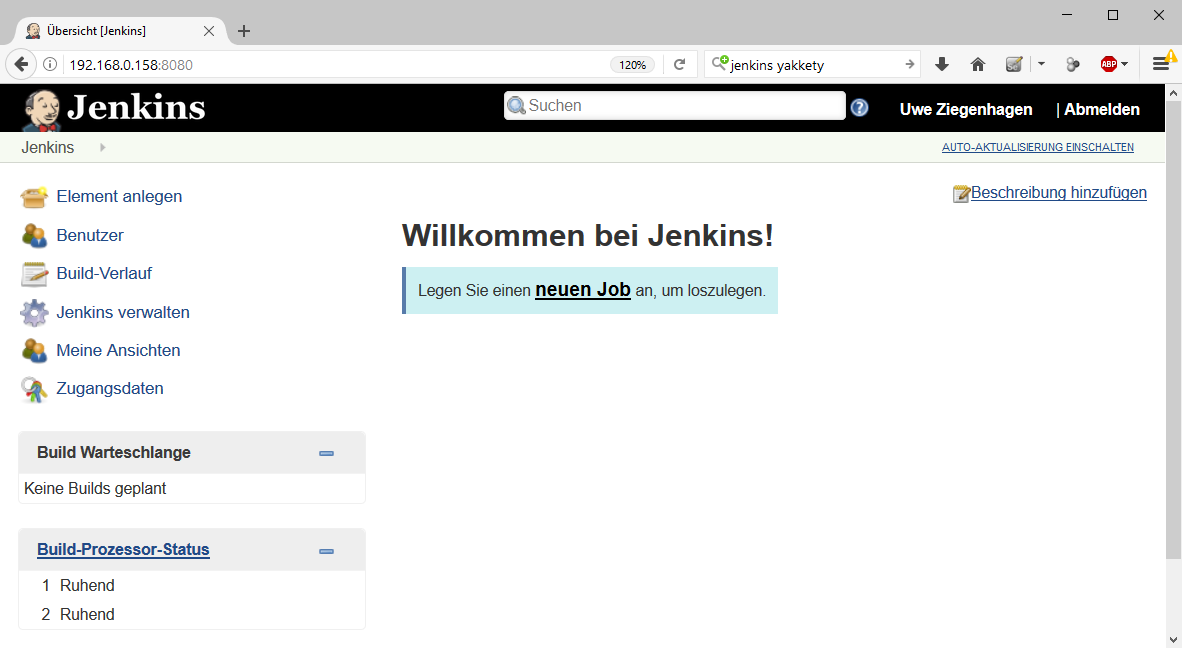
\includegraphics[width=\textwidth]{Images/NewJob}}
\caption{Die jenkins-Oberfläche}\label{fig:NewJob}
\end{figure}

